%------------------------------------------------
\begin{frame}
\frametitle{Le chiffrement}
\justifying{
\begin{block}{En local - ses données}
\begin{itemize}
\item Son disque dur
\item Sa clef USB
\item Son smartphone
\end{itemize}
\end{block}

\begin{block}{En réseau - ses communications}
\begin{itemize}
\item Https : utilisation de l'extension HTTPSEveryWhere pour Firefox  
\item Ses e-mails : utilisation de GPG via Enigmail pour Thunderbird
\item Sa connexion : utiliser un VPN, SSH, la clef "WIFI".
\end{itemize}
\end{block}

\begin{block}{}
$\Rightarrow$ \`A chaque "usage", il y a une solution de chiffrement possible.
\end{block}
}
\end{frame}


%----------------------------------------------------------------------------------------
\begin{frame}
\frametitle{Les mails - PGP, GPG?}
\begin{block}{PGP}
\justifying{
Pretty Good Privacy - PGP est un logiciel de chiffrement et de déchiffrement cryptographique, créé par l'américain Phil Zimmermann en 1991.
}
\end{block}
\begin{block}{OpenPGP}
\justifying{
Ce standard décrit le format des messages, signatures ou certificats que peuvent s'envoyer des logiciels comme GNU Privacy Guard. Ce n'est donc pas un logiciel, mais un format pour l'échange sécurisé de données, qui doit son nom au programme historique Pretty Good Privacy (PGP).
}
\end{block}
\begin{block}{GnuPG}
\justifying{GnuPG (ou GPG, de l'anglais GNU Privacy Guard) est l'implémentation GNU du standard OpenPGP.}
\end{block}
\end{frame}


%----------------------------------------------------------------------------------------
\begin{frame}

\frametitle{Chiffrer son disque dur}
\begin{block}{Logiciels intégrés aux systèmes d'exploitations}
\begin{itemize}
\item Windows 7/8 : Bitlocker (Backdor)
\item MacOS : FileVault
\item GNU/Linux : Encfs...
\end{itemize}
Peut-on faire confiance à autre chose que du logiciel libre ?
\end{block}

\begin{block}{Indépendament du système d'exploitation}
$\Rightarrow$ Le logiciel TrueCrypt. Pour une clef USB/un disque dur externe.
\end{block}
\end{frame}

%----------------------------------------------------------------------------------------
\begin{frame}
\frametitle{L'audit de TrueCrypt}
\begin{center}
 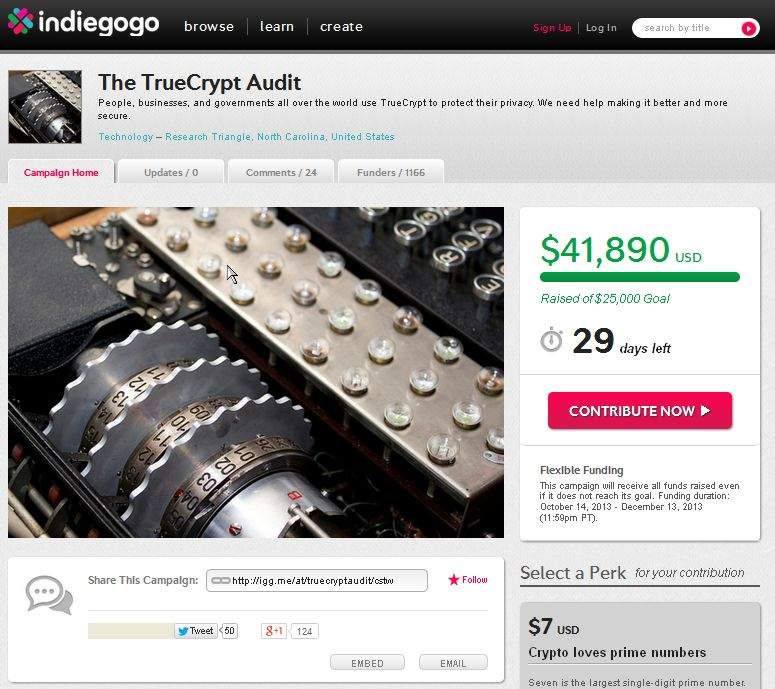
\includegraphics[scale=0.45] {./materials/truecryptaudit.jpg} 
\end{center}
\end{frame}
